\documentclass{article}

\usepackage{generalsnips}
\usepackage{calculussnips}
\usepackage[margin = 1in]{geometry}
\usepackage{pdfpages}
\usepackage[spanish]{babel}
\usepackage{amsmath}
\usepackage{amsthm}
\usepackage[utf8]{inputenc}
\usepackage{titlesec}
\usepackage{xpatch}
\usepackage{fancyhdr}
\usepackage{tikz}
\usepackage{hyperref}
\usepackage{float}
\title{Price Discrimination}
\date{2020 April 12, 08:09PM}
\author{David Gabriel Corzo Mcmath}

\begin{document}
\maketitle
%%%%%%%%%%%%%%%%%%%%%%%%%%%%%%%%%%%%%%%%%%%%%%%%%%%%%%%%%%%%%%%%%%%%%%%%%%%%%%%%%%%%%%%%%%%%%%%%%%%%%%%%%%%%%%%%%%%%%%%%%%%%%%%%%%%%%%%%%%%%%%

\section{Price Discrimination}
\termdefinition{Price Discrimination}{Selling the same product at diferent groups of customers at diferent prices.}

%----------------------------------------------------------------------------------------
\subsection{Introduction}
Conclution: Price discrimination maximizes profits.
\begin{figure}[H]
    \centering
    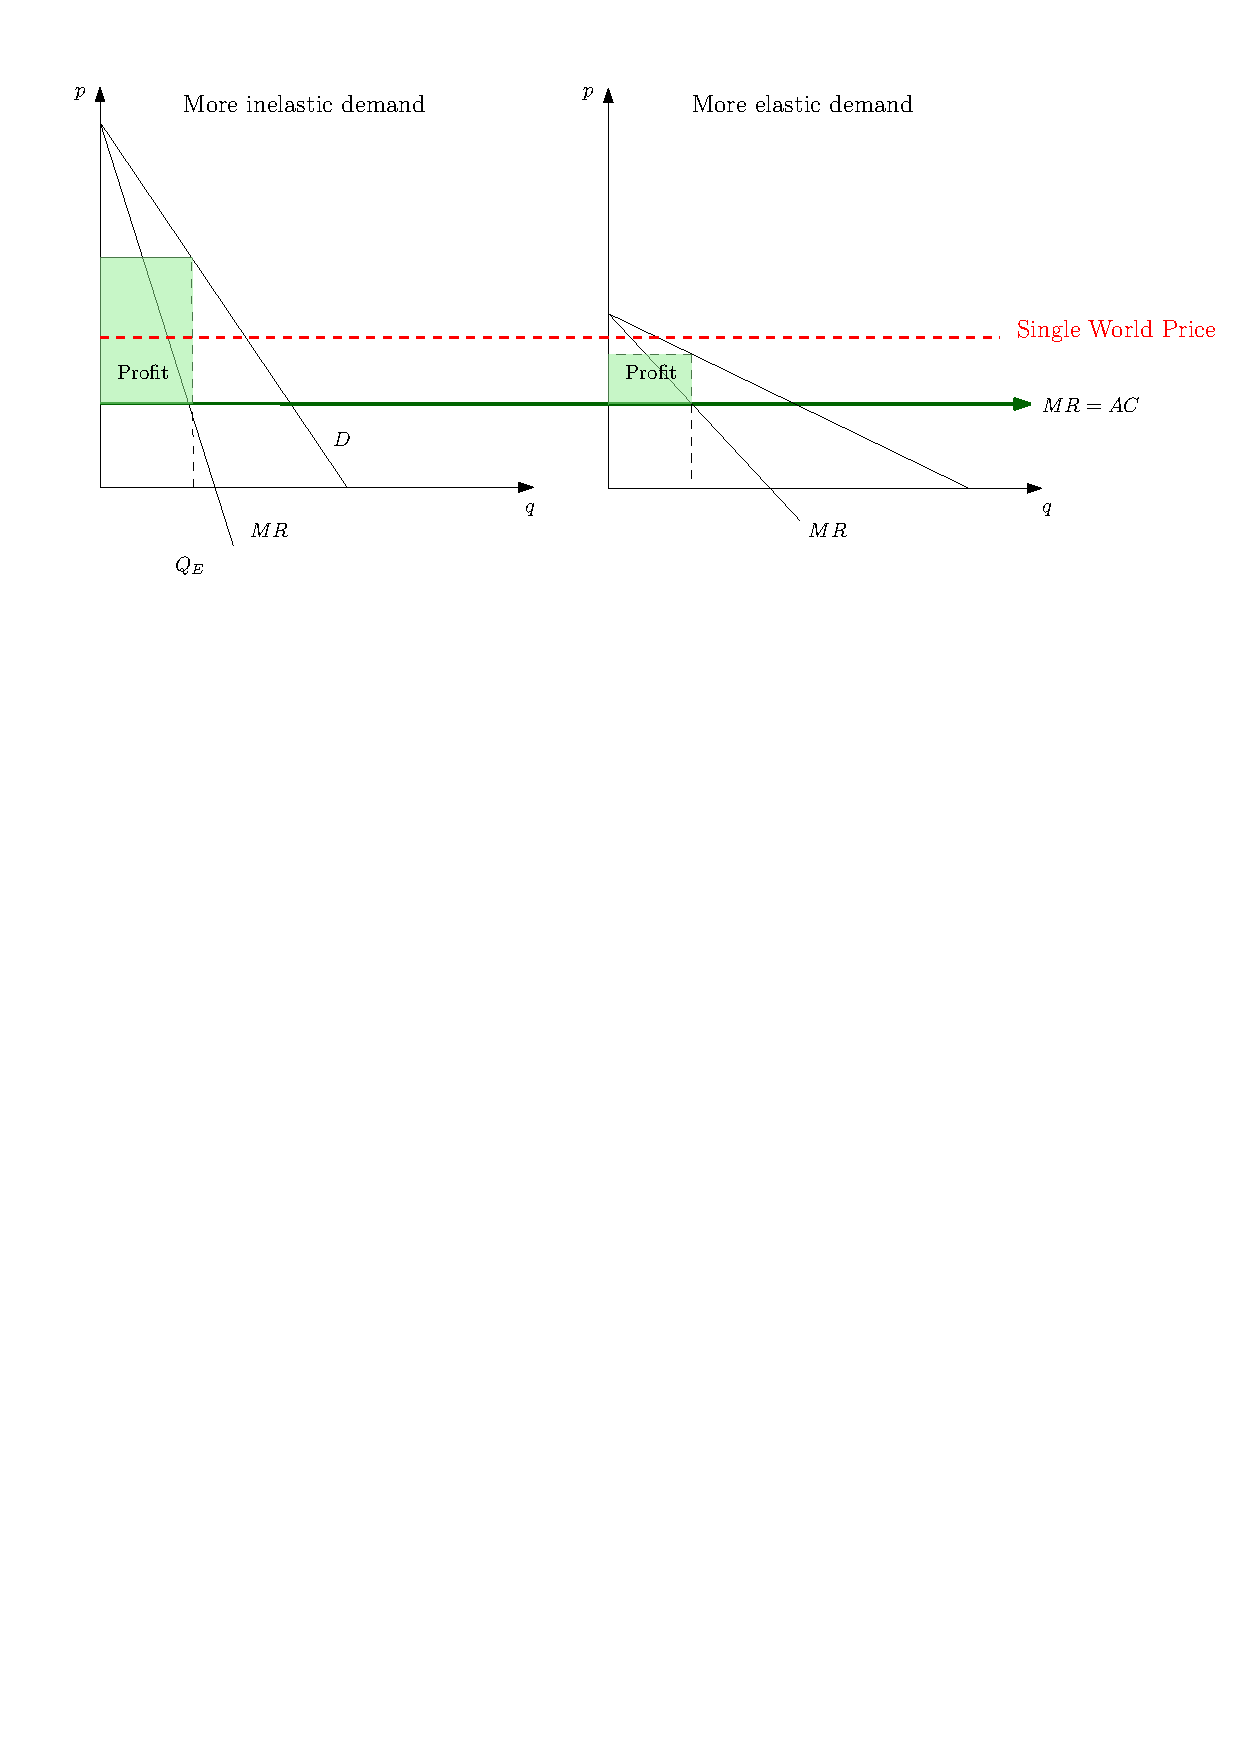
\includegraphics[width=17cm]{figs/price_discrimination.pdf} 
\end{figure}

%----------------------------------------------------------------------------------------
\subsection{Price discrimination principles}
\begin{enumerate}
    \item If demand curves are different, it is more profitable to set diferent prices in diferent markets.
        \begin{itemize}
            \item The price should be higher in the market with more inelastic demand.
        \end{itemize}
    
    \item Arbitrage (makes the prices in the two markets closer together) makes it more difficult to price discriminate. 
\end{enumerate} 


%----------------------------------------------------------------------------------------
\subsection{Markets can be segmented in more ways than geographically}
By segmenting the market you can price discriminate. For example:
\begin{itemize}
    \item Masouses
    \item Movie theaters
    \item Computer Software 
    \item Airlines 
\end{itemize}


%----------------------------------------------------------------------------------------
\subsection{Discrimination is hard}
Distinglishing between market segments are hard and difcult to determine, but when they are determined is because of a caracteristics. 



%----------------------------------------------------------------------------------------
\section{The birth and death of the price tag}
\begin{itemize}
    \item Coca cola tries to price discriminate.
    \item Quakers are against price discrimination. 
    \item The price tag is invented with the objective of having really big stores. 
    \item The death of the price tag started with air faires. 
    \item Airlines have mastered the art of price discrimination. 
    \item People fear the idea that things they need will increase in price. 
\end{itemize}



%%%%%%%%%%%%%%%%%%%%%%%%%%%%%%%%%%%%%%%%%%%%%%%%%%%%%%%%%%%%%%%%%%%%%%%%%%%%%%%%%%%%%%%%%%%%%%%%%%%%%%%%%%%%%%%%%%%%%%%%%%%%%%%%%%%%%%%%%%%%%%
\end{document}

